\subsection{Problem Definition}

The following problem deals with simulating fluid flow and heat transport in a 3 dimensional heterogeneous faulted geological system.  
%figure1
\label{sec:model}
\begin{figure}[htbp]
    \begin{center}
        \includegraphics[width=0.40\textwidth]{T/figures/2u2f_fig1.eps}
        \caption{Sample model consisting of two geological layers cut by a system of two crossing faults.}
        \label{fig1}
    \end{center}
\end{figure}

The model volume consists of two sub-horizontal geological layers, including two dipping faults (Figure \ref{fig1}). The horizontal north-south and east-west extensions are 200 m, resulting in a horizontal model area of 40,000 m$^{2}$. The two geological layers are vertically bordered by three curved surfaces. The elevation of top, middle and bottom surface is 55 m $\pm{}$ 5m, 0 m $\pm{}$ 7 m and -45 m $\pm{}$ 5 m, respectively.  Therefore, an average thickness of 55 m for layer 1 and 45 m for layer 2 is established (Table \ref{tab:geometry}).

%table1
\begin{table}[htbp]
    \begin{center}
        \caption{Geometrical attributes of the geological layers and faults.}
        \begin{tabular}{lccc}
          \hline
          property & unit & layer1 & layer2\\
          \hline
          \hline
          average thickness $t$ & [m] & 55 & 45\\
          \hline
                   &      & fault1 & fault2\\
          \hline
          \hline
          dip direction & [$^\circ$] & 316.7 & 225\\
          dip & [$^\circ$] & 80.6 & 63.2\\
          length $l$ & [m] & 233.5 & 183.8\\
          \hline        
        \end{tabular}
        \label{tab:geometry}
    \end{center}
\end{table}

Both faults are penetrating the two geological layers. Fault 1 has a length of 233 m and is striking North-East, with dip coordinates of 316.7$^\circ{}$; 80.6$^\circ{}$. Fault 2 has a length of 184 m and  is oriented perpendicular to fault 1, having dip coordinates of 225$^\circ{}$; 63.2$^\circ{}$ (Table \ref{tab:geometry}).

\subsection{Initial and boundary conditions}
%figure2
\begin{figure}[htbp]
    \begin{center}
        \includegraphics[width=0.48\textwidth]{T/figures/2u2f_fig2.eps}
        \caption{Pressure boundary condition of the sample model.}
        \label{fig2}
    \end{center}
\end{figure}
During the simulation, a general flow field from the South to the North is generated. Dirichlet (or first-type) boundary conditions for pressure are set along the southern and northern boundaries (Figure\ref{fig2}). According to the definition of hydrostatic pressure, the pressure at the southern border is constant at p(x, y = -100 m, z) = $\rho{}$gz + 1.75$\cdot10^{6}$ Pa and at the northern border at p(x, y = 100 m, z) = $\rho{}$gz + 1.25 $\cdot10^{6}$ Pa (Figure \ref{fig2}), where $\rho{}$ [1000 kg/m$^{3}$], g [9.81 m/s$^{2}$] and z denotes the fluid density, gravitational acceleration and height of liquid column, respectively. An average hydraulic gradient $\nabla{}$h = 5$\cdot10^{5}$ Pa / 200 m = 0.25 from the South to the North is provided. For the remaining domain, a pressure value of 1.75$\cdot10^{6}$ Pa is initialized. 
%figure 3
\begin{figure}[htbp]
    \begin{center}
        \includegraphics[width=0.48\textwidth]{T/figures/2u2f_fig3.eps}
        \caption{Temperature boundary conditions of the sample model.} 
        \label{fig3}
    \end{center}
\end{figure}

To generate an inflow of hot and cold water from the southern border, Dirichlet boundary conditions for temperature are applied too (Figure \ref{fig3}). Along the southern border, temperature increases from 40$^\circ{}$C to 80$^\circ{}$C, in going from West to the East resulting in a temperature profile of T (x, y = -100 m, z) = 0.2$^\circ{}$C/m * x + 60$^\circ{}$C (Figure \ref{fig3}). For the remaining domain, the initial temperature is set to 60$^\circ{}$C.

\subsection{Parameters}

Table \ref{tab:layers} shows the hydraulic properties of the two geological layers.
%table2
\begin{table}[htbp]
    \begin{center}
        \caption{Porous medium properties of geological layers.}
        \begin{tabular}{lccc}
          \hline
          property & unit & layer1 & layer2\\
          \hline
          \hline
          porosity $\phi{}$ & [-] & 0.15 & 0.08\\
          storage $\beta{}$ & [1/Pa] & 7$\cdot10^{-10}$ & 7$\cdot10^{-10}$\\
          permeability $k$ & [m$^{2}$] & 2$\cdot10^{-14}$ & $10^{-14}$\\
          \hline
        \end{tabular}
        \label{tab:layers}
    \end{center}
\end{table}

To assure a variation of the hydraulic properties, the upper geological layer was modeled twice as conductive as the lower layer. The permeability $k$ of layer 1 is set to 2$\cdot10^{-14}$ m$^{2}$ and the porosity  $\phi{}$ to 0.15. For layer 2 the permeability k is set to $10^{-14}$ m$^{2}$ and the porosity $\phi{}$ to 0.08. The storage of both layers is derived from the bulk compressibility $\beta{}$ [1/Pa] of the rock and the embedded fluid. Assuming fissured rocks, the storage is set to 7$\cdot10^{-10}$ 1/Pa.

In table \ref{tab:faults} the relevant parameters for the system of the two faults are listed.
%table3
\begin{table}[htbp]
    \begin{center}
        \caption{Medium properties of faults.}
        \begin{tabular}{lccc}
          \hline
          property & unit & fault1 & fault2\\
          \hline
          \hline
          aperture $a$ & [m] & .05 & .05\\
          porosity $\phi{}$ & [-] & 1 & 1\\
          storage $\beta{}$ & [1/Pa] & 4.6$\cdot10^{-10}$ & 4.6$\cdot10^{-10}$\\
          permeability $k$ & [m$^2$] & $10^{-8}$ & 5$\cdot10^{-9}$\\
          \hline
        \end{tabular}
        \label{tab:faults}
    \end{center}
\end{table}

The permeability of fault 1 is set to $10^{-8}$ m$^{}$ and that of fault 2 to 5$\cdot10^{-9}$ m$^{2}$. The fault transmissivity is defined as the product of the fault permeability $k$ and aperture $a$. To ensure a high contrast between fault transmissivity and matrix conductivity, the aperture of both faults is set to 0.05 m. To provide free fluid flow in the faults, a porosity value of 1.0 is chosen. The storage in the faults is due to the fluid compressibility only and $\beta{}$  = 4.6$\cdot10^{-10}$ 1/Pa is assigned.

The simulation time is set to 145 years in order to observe in the simulation the major changes characterizing the temperature field. 

\subsection{Results}
\label{sec:results}

After approximately one month a steady state for pressure and velocity field is achieved (Figure \ref{fig4}).
%figure4
\begin{figure}[htbp]
    \begin{center}
        \begin{minipage}{0.40\textwidth}
            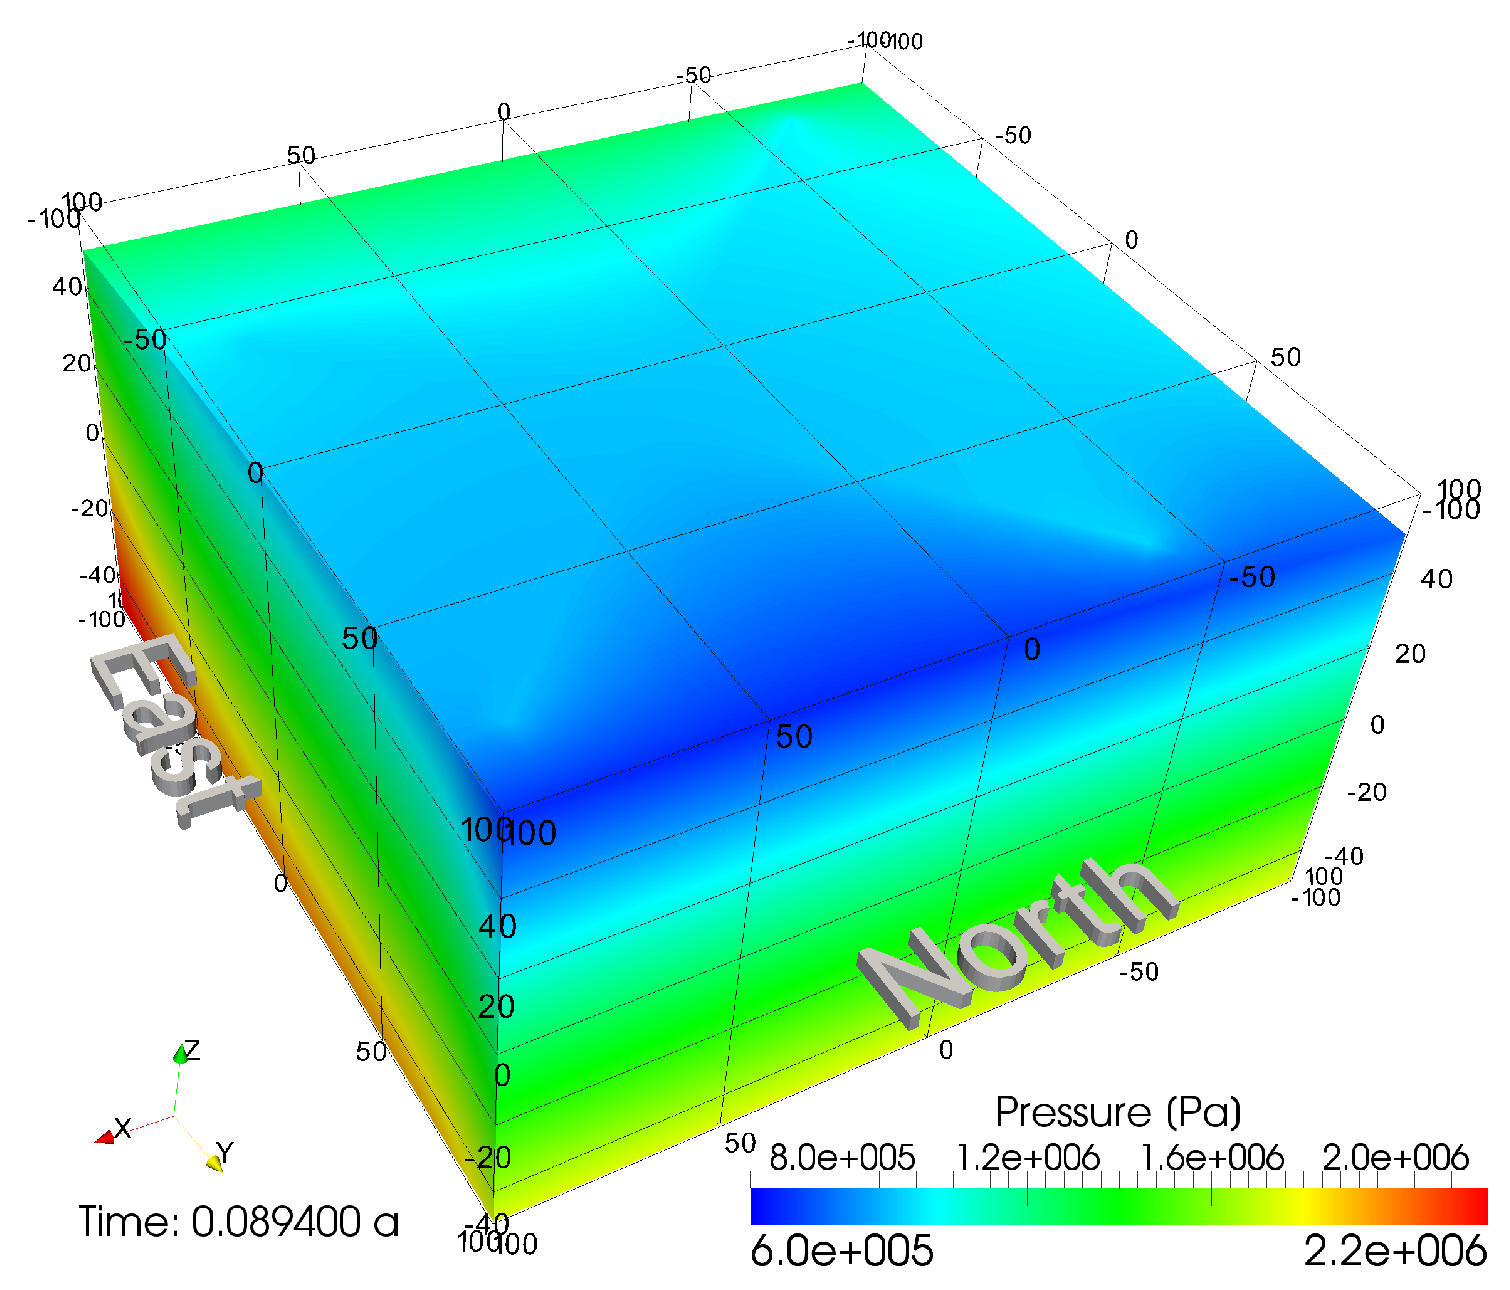
\includegraphics[width=1\textwidth]{T/figures/2u2f_fig4a.eps}
        \end{minipage}
        \begin{minipage}{0.40\textwidth}
            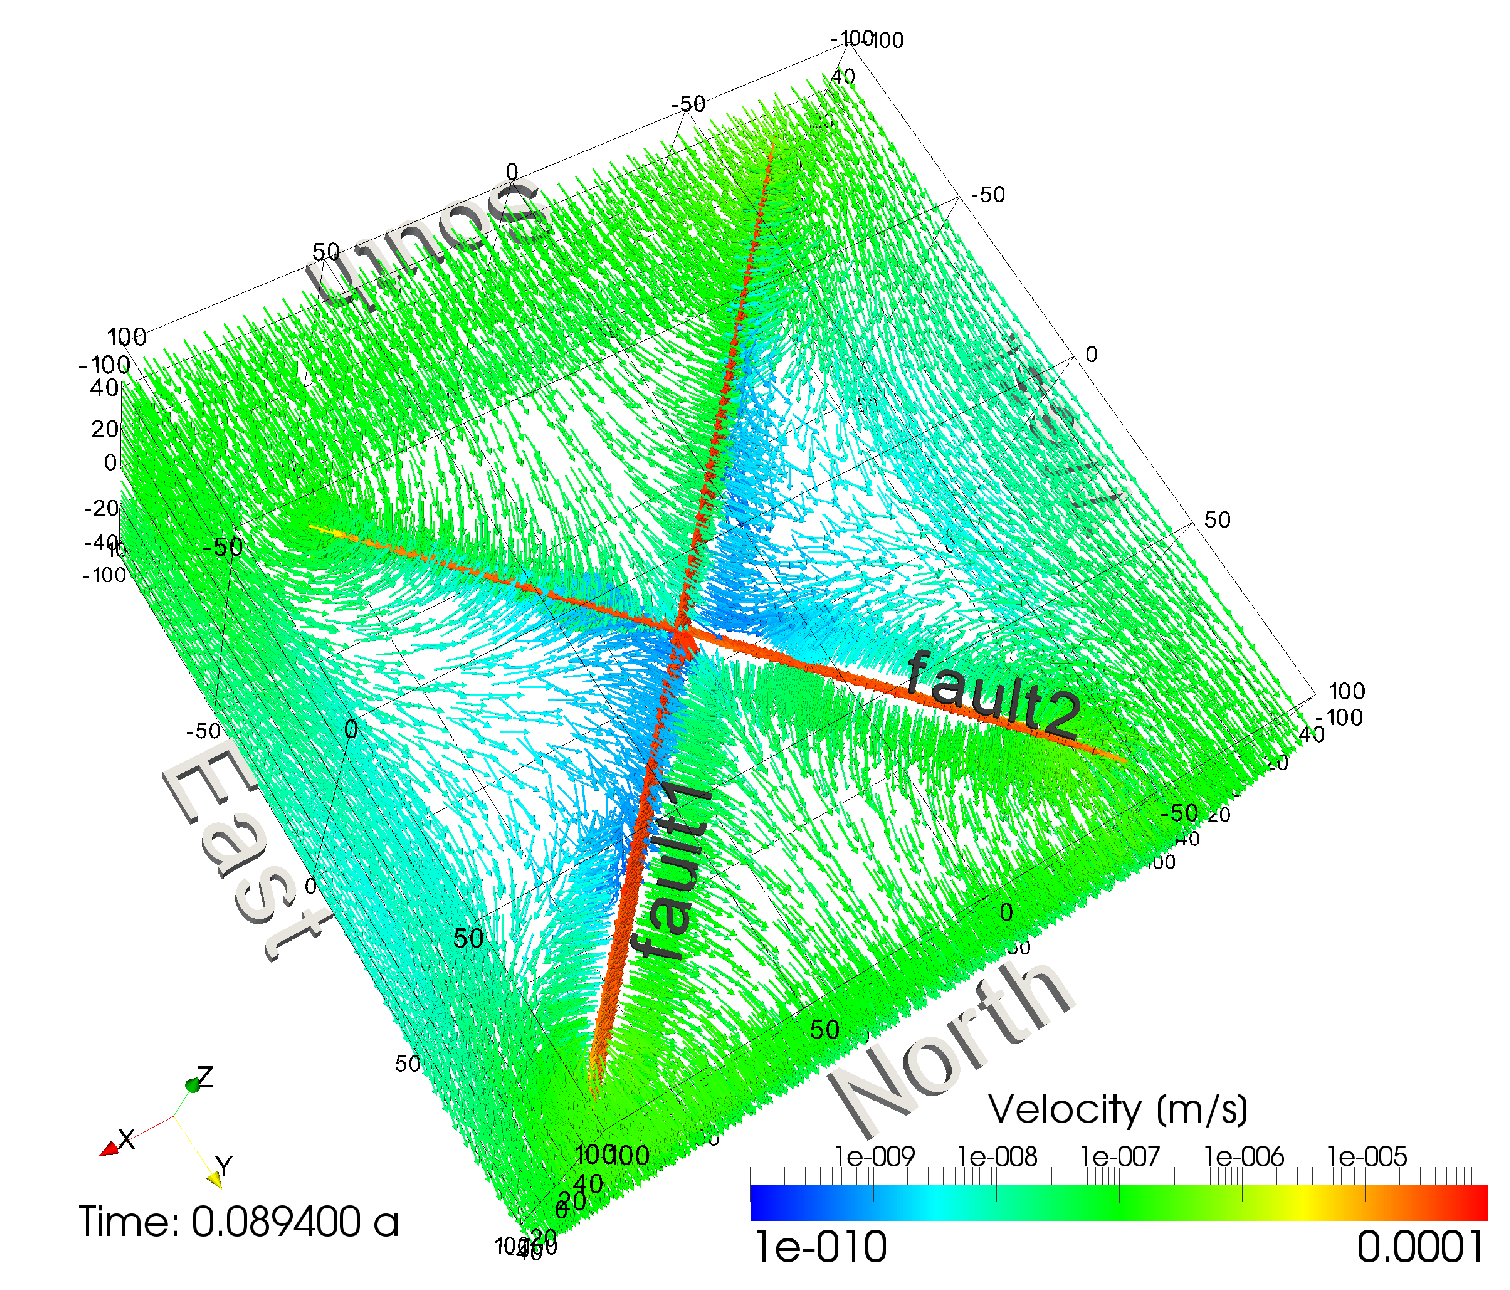
\includegraphics[width=1\textwidth]{T/figures/2u2f_fig4b.eps}
        \end{minipage}
        \caption{Simulated steady pressure (\ref{fig4}a) and velocity field (\ref{fig4}b) achieved after approx. 1 month.}
        \label{fig4}
    \end{center}
\end{figure}

Due to the fact that the implemented faults do not cut the southern and northern borders of the model, matrix flow is predominant in these areas. Accordingly, the highest pressure gradients are observed at the northern and southern borders of the model (Figure \ref{fig4}a). In proximity to the cutting faults, the isobars (surfaces of constant pressure) are sub-horizontal due to high flow rates within the faults. Maximum Darcy velocities of v = $\cdot10^{-4}$ m/s can be observed inside the faults (Figure \ref{fig4}b). Despite low pressure gradients, high flow rates occur in the fault planes. High values of fluid velocity are the result of the relative high transmissivity of the faults with respects to the surrounding domain.

Figure \ref{fig4}b shows the stationary flow field. As described above, highest flow velocities can be observed in the fault planes. The applied pressure boundary conditions force a regional flow field from the South to the North. The average velocity at the southern and northern regions is $10^{-7}$ m/s, with maximum inflow to the faults from the South. In the rest of the domain, outflow from the faults into the rock matrix is pronounced. In the central part of the model, faults act as the predominant flow paths. In contrast, low velocities (less than $10^{-8}$ m/s) characterize the eastern and western boundaries. An additional important fact is that at the southern edge of fault 1 and fault 2, backward flow from the North to the South occurs. Pressure equalisation within the faults results in higher matrix pressure at this area. This causes drainage of the rock matrix by the fault system.

Figure \ref{fig5}a-\ref{fig5}d shows the 45$^\circ{}$C, 55$^\circ{}$C, 65$^\circ{}$C and 75$^\circ{}$C contours at four different time stages.

%figure5
\begin{figure}[htbp]
    \begin{center}
        \begin{minipage}{0.35\textwidth}
            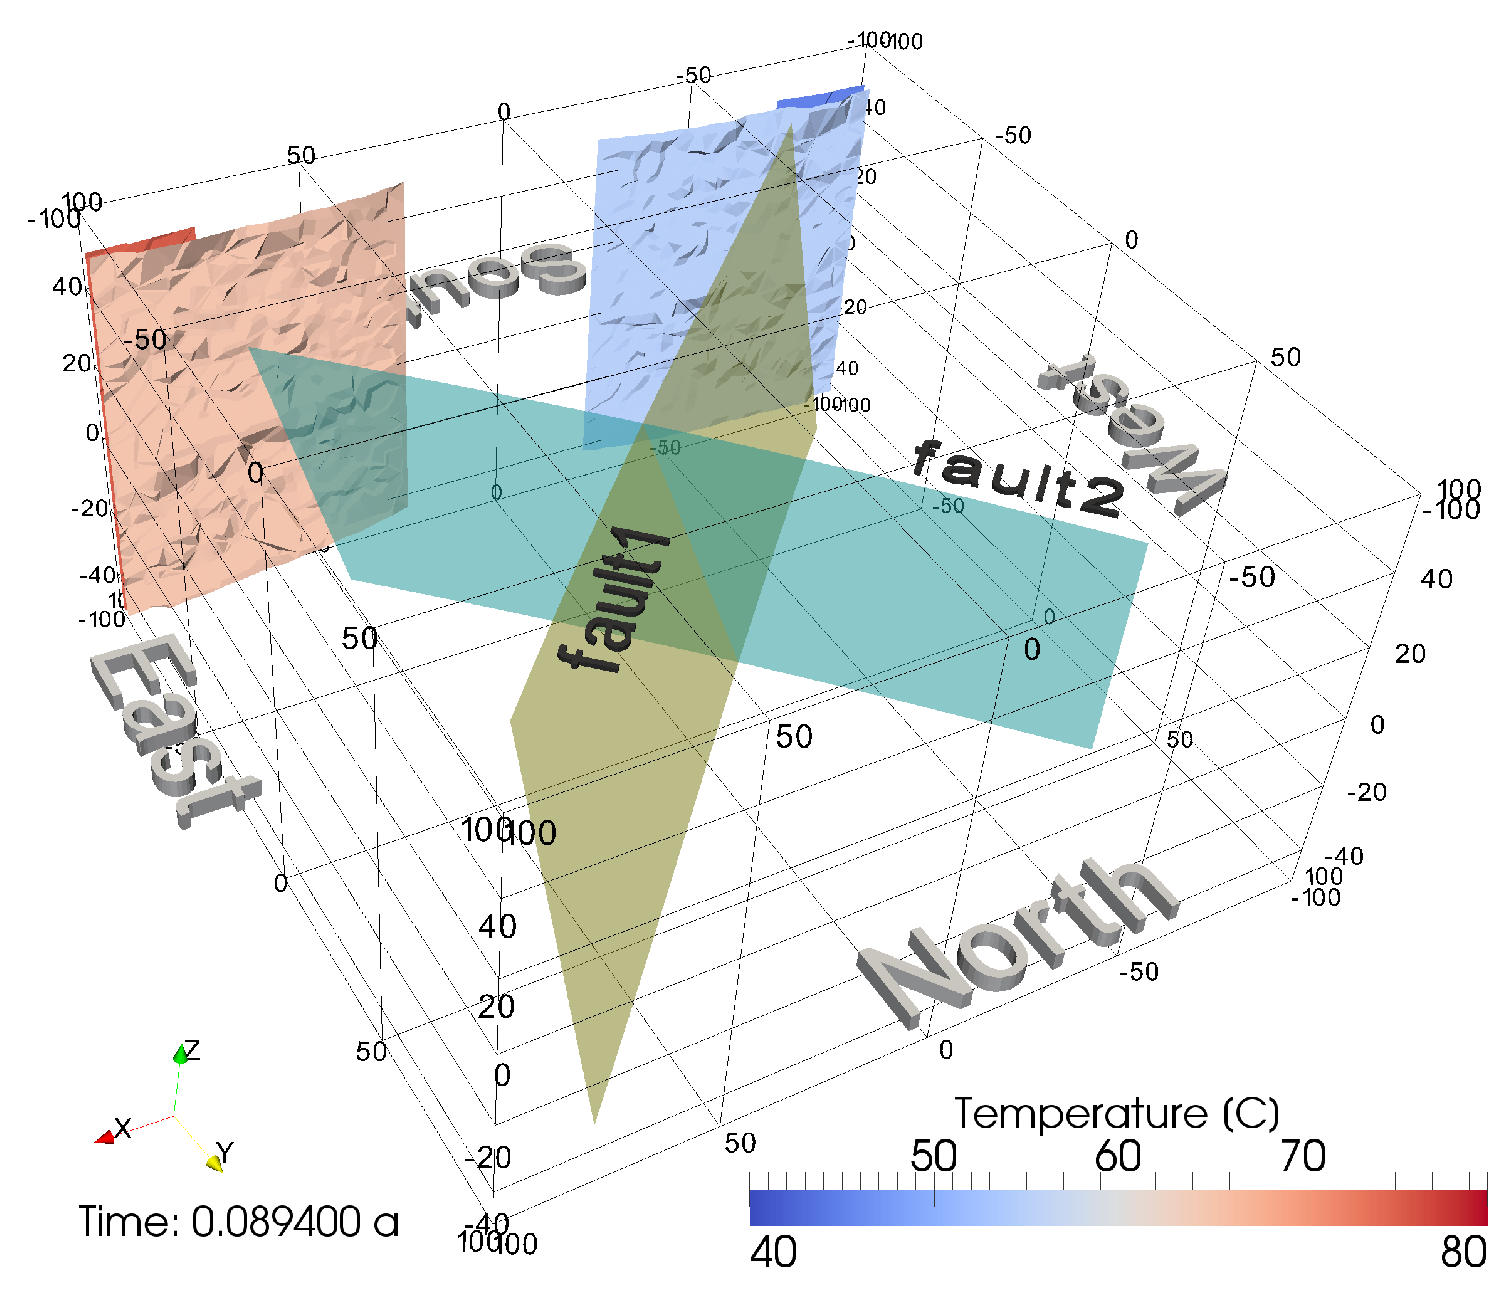
\includegraphics[width=1\textwidth]{T/figures/2u2f_fig5a.eps}
        \end{minipage}
        \begin{minipage}{0.35\textwidth}
            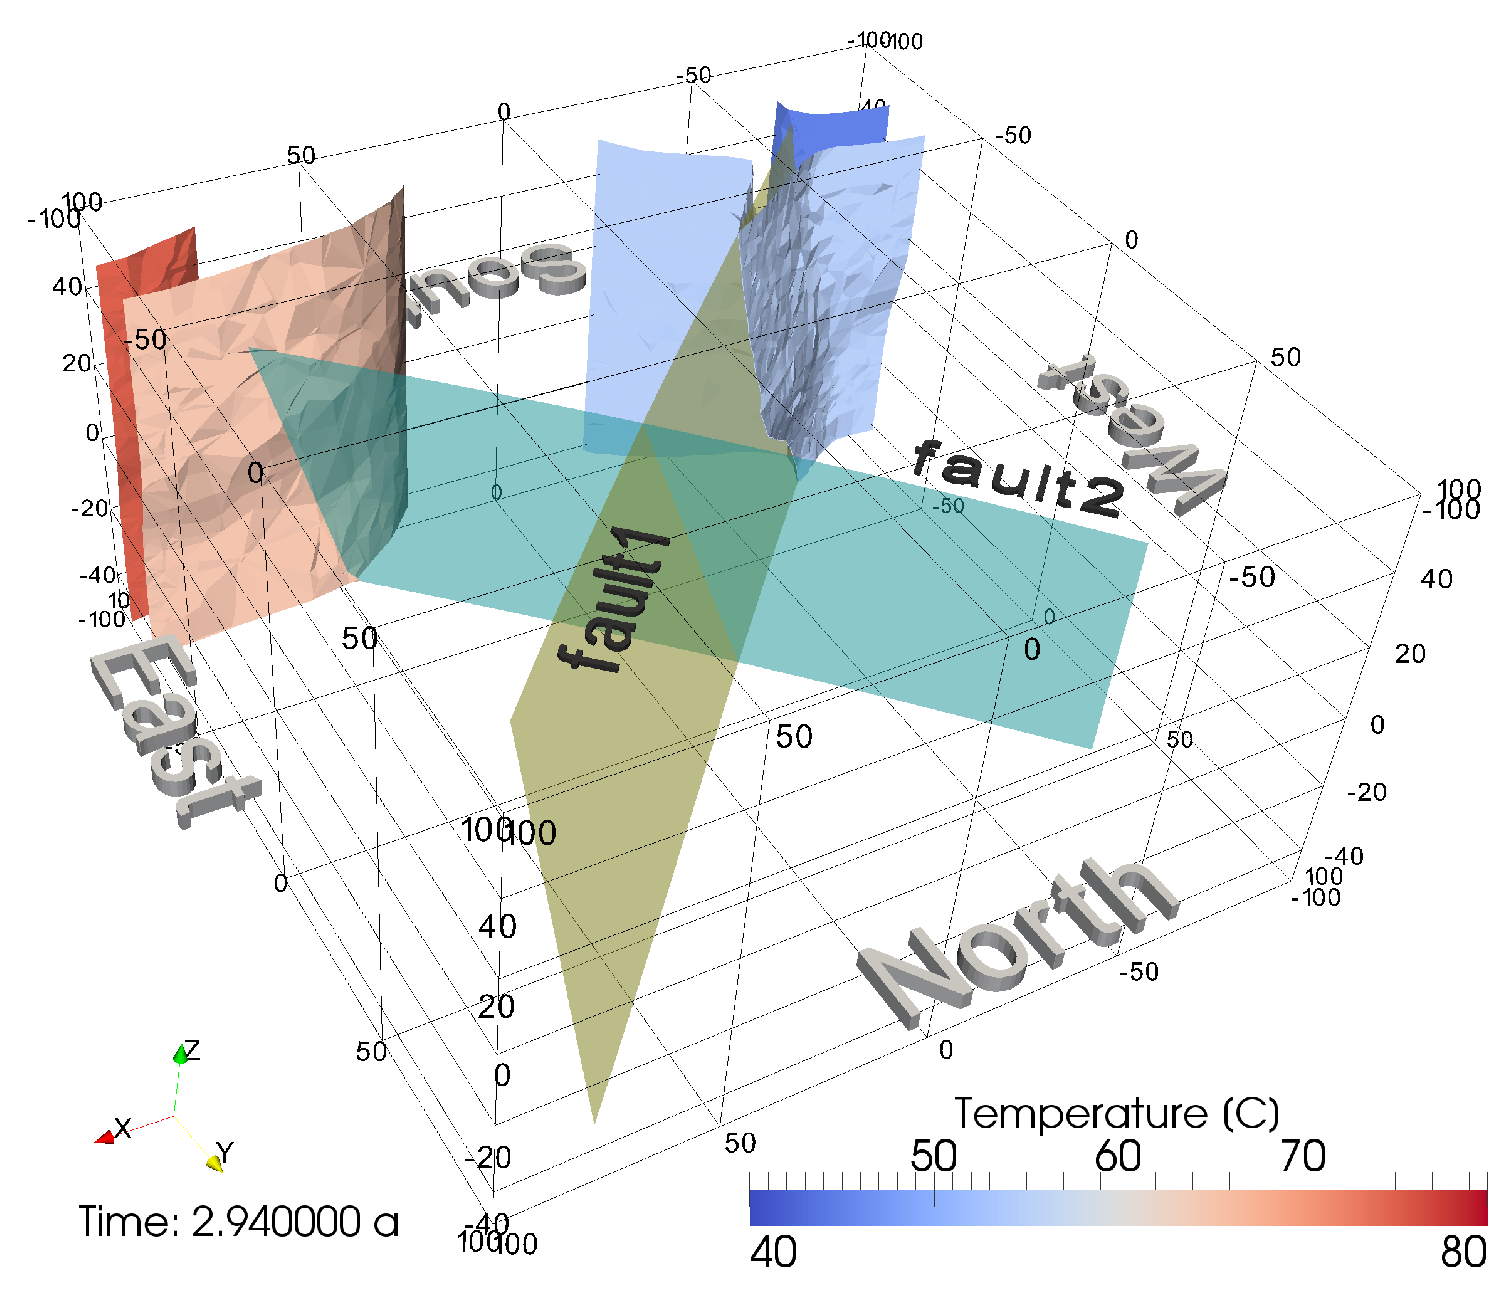
\includegraphics[width=1\textwidth]{T/figures/2u2f_fig5b.eps}
        \end{minipage}
        \begin{minipage}{0.35\textwidth}
            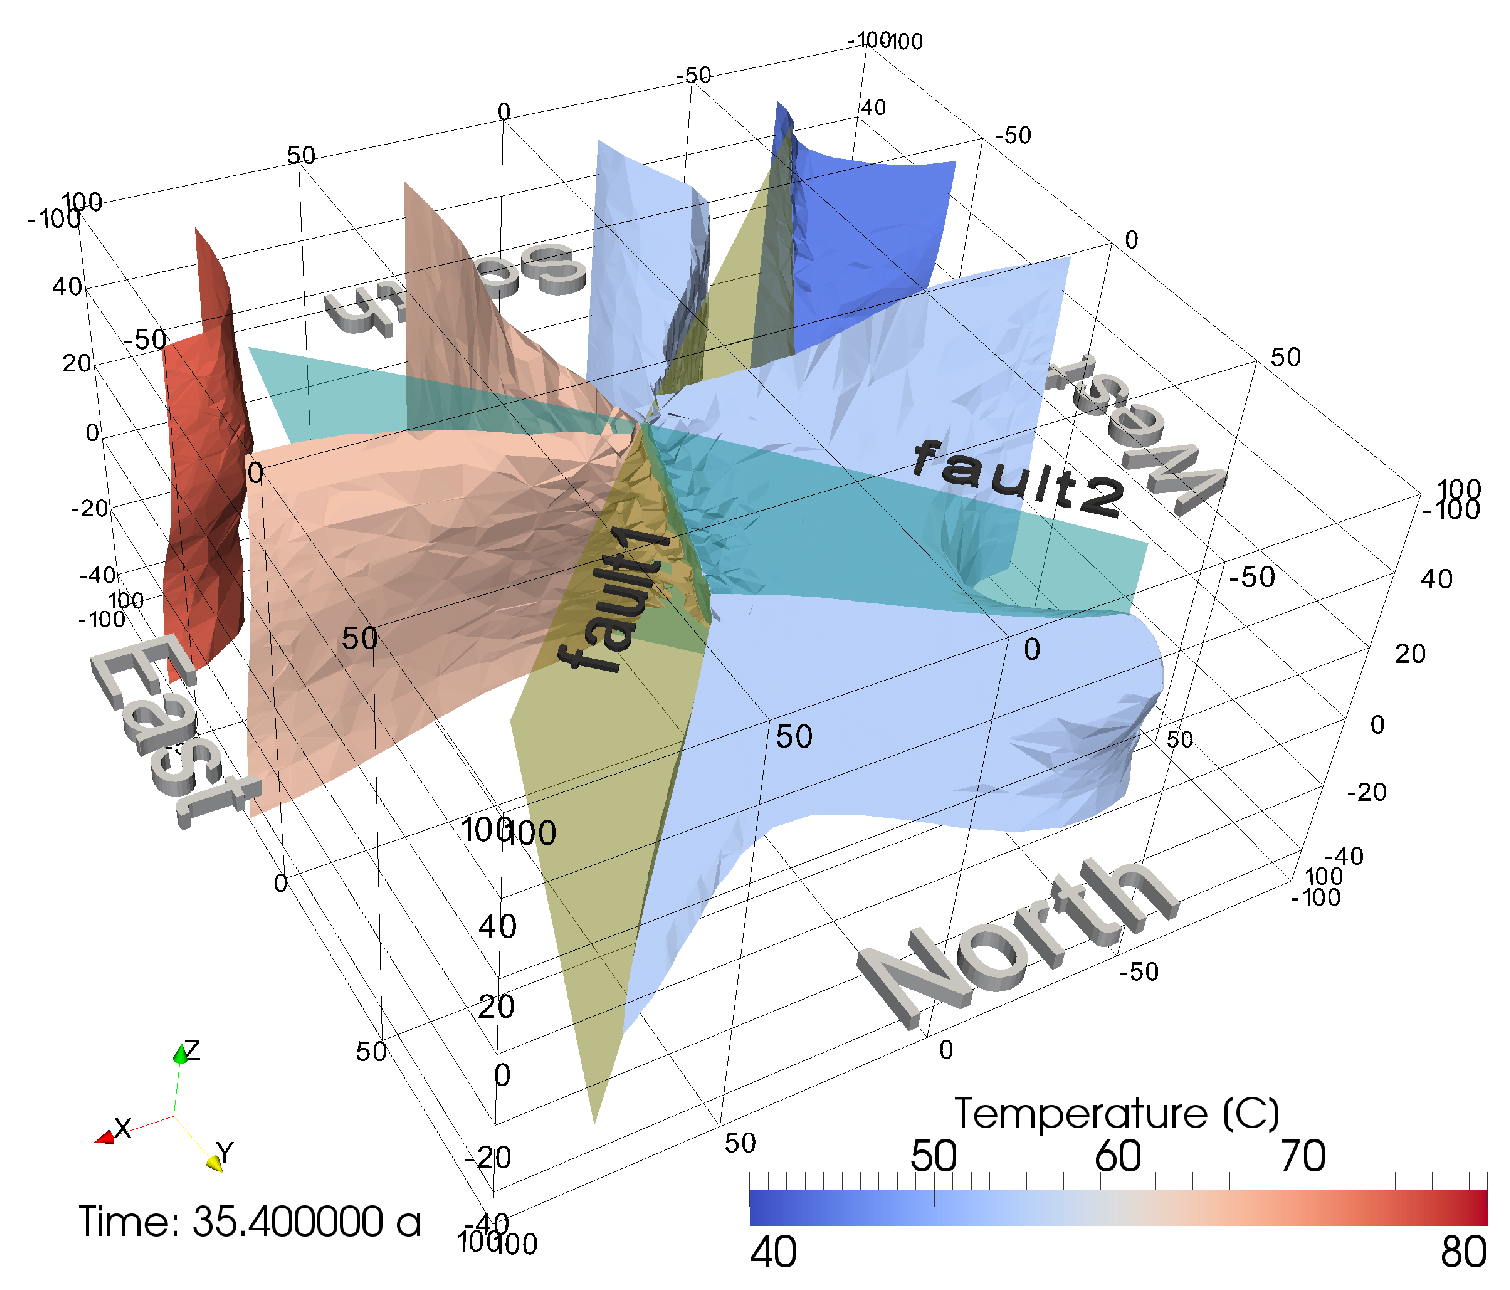
\includegraphics[width=1\textwidth]{T/figures/2u2f_fig5c.eps}
        \end{minipage}
        \begin{minipage}{0.35\textwidth}
            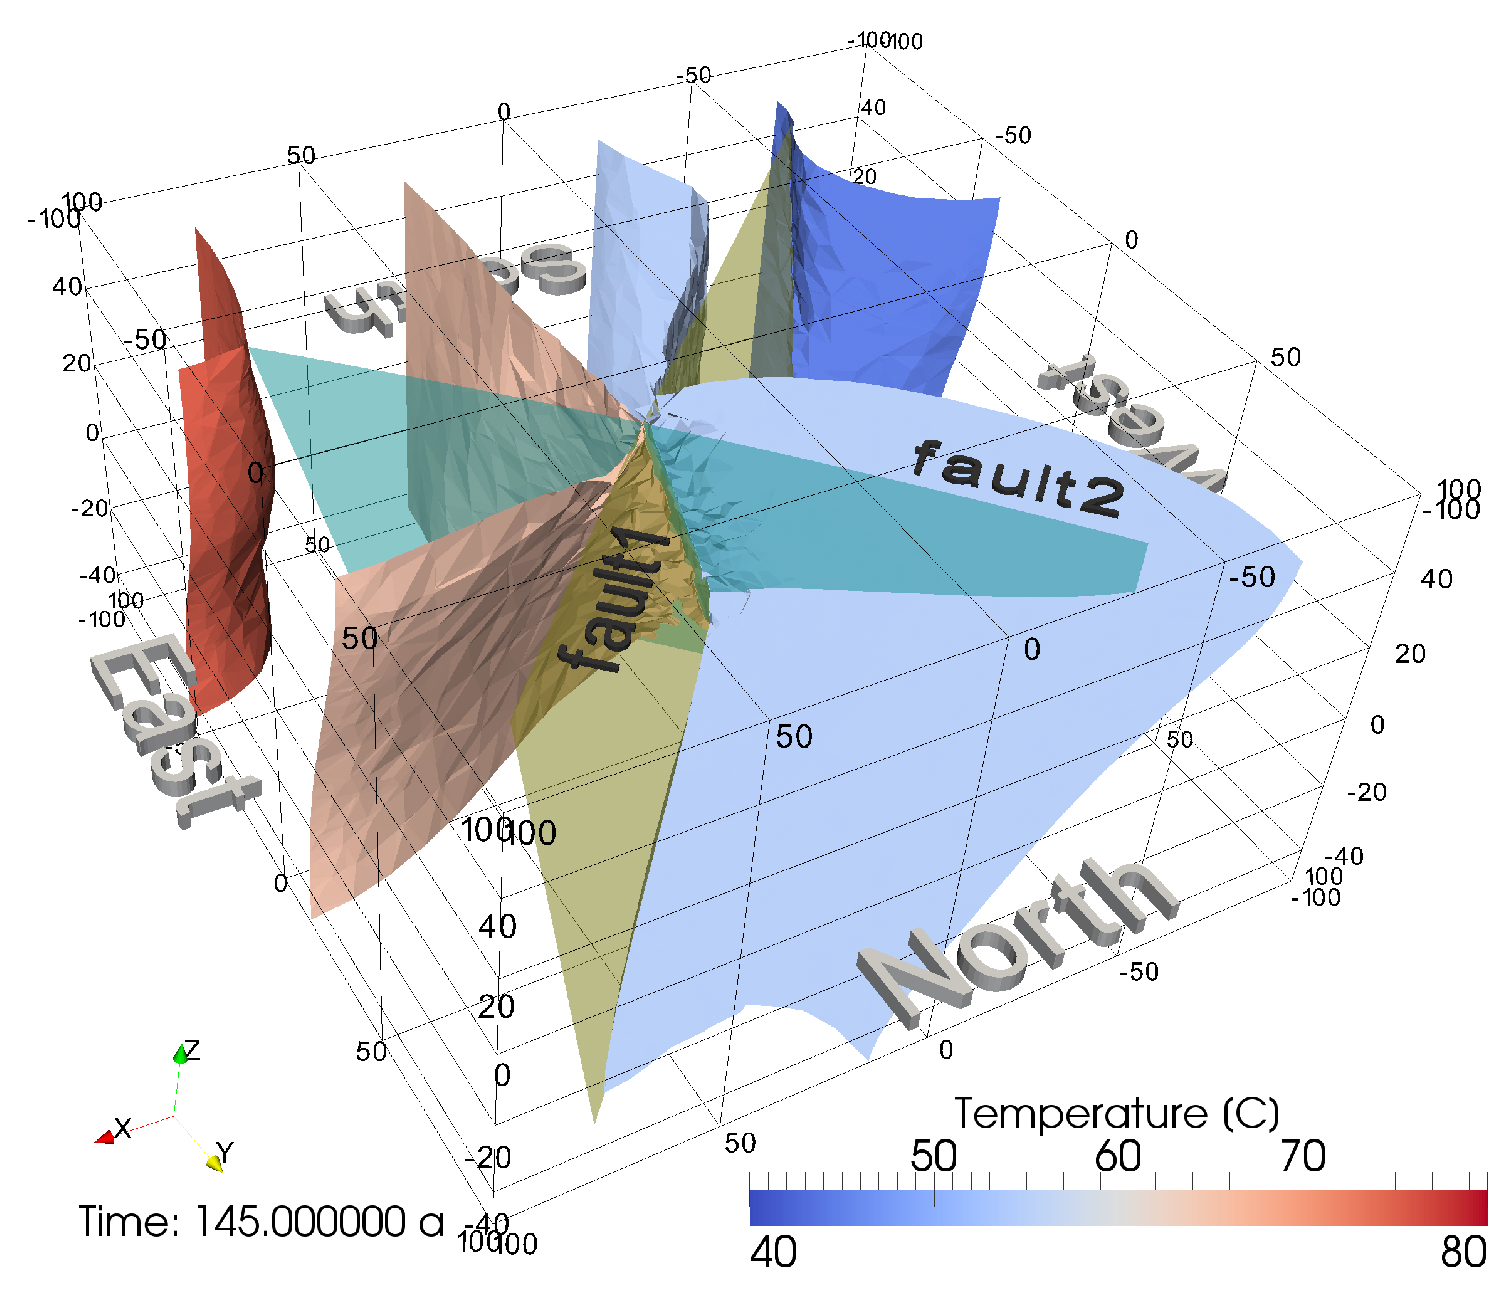
\includegraphics[width=1\textwidth]{T/figures/2u2f_fig5d.eps}
        \end{minipage}
        \caption{Temperature contour plots (45$^\circ{}$C, 55$^\circ{}$C, 65$^\circ{}$C and 75$^\circ{}$C isosurfaces) at four different time stages.}
        \label{fig5}
    \end{center}
\end{figure}

Before stationary field conditions for pressure and velocity are reached, conductive heat transfer does not affect the initial temperature field significantly (Figure \ref{fig5}a). After achieving the stationary pressure and velocity field, convective heat transfer (advection plus diffusion) becomes predominant. The cold water front (T = 55$^\circ{}$C) enters fault 1 after approx. 4 months (Figure \ref{fig5}b). Due to the geometry of fault 1 with respects to the southern boundary of the domain, cold water enters fault 1 in the upper part. After 35 years, (Figure \ref{fig5}c) cold water from fault 1 and hot water from fault 2 are mixed at the fault intersection. The final temperature field (Figure \ref{fig5}d) shows an average temperature of T = 55$^\circ{}$C in the northern part which is less than the mean initial temperature of 60$^\circ{}$C. The depression from the mean value is caused because fault 1 is more conductive than fault 2, which drives higher amounts of cold water into the system.

For a detailed observation of the pressure, velocity and temperature evolution inside the two faults, three observation points were set (Figure \ref{fig6}a).

%figure6
\begin{figure}[htbp]
    \begin{center}
        \begin{minipage}{0.40\textwidth}
            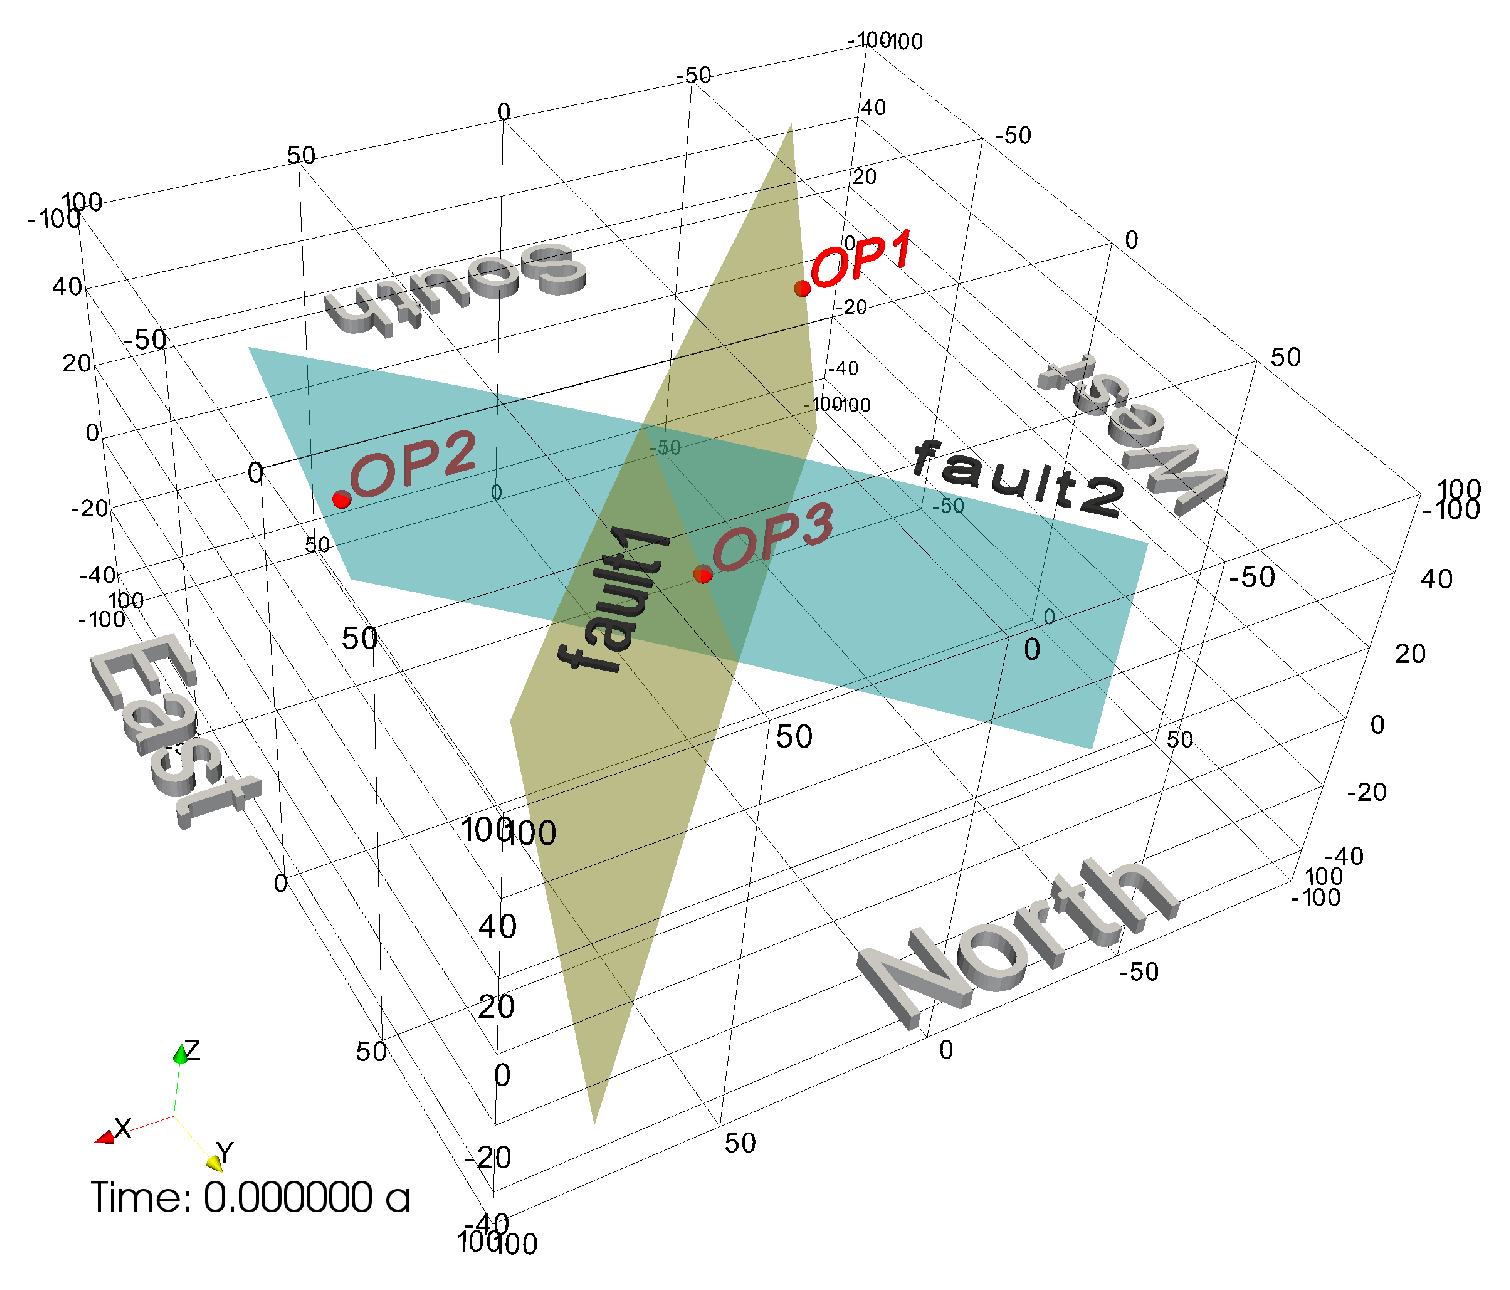
\includegraphics[width=1\textwidth]{T/figures/2u2f_fig6a.eps}
        \end{minipage}
        \begin{minipage}{0.40\textwidth}
            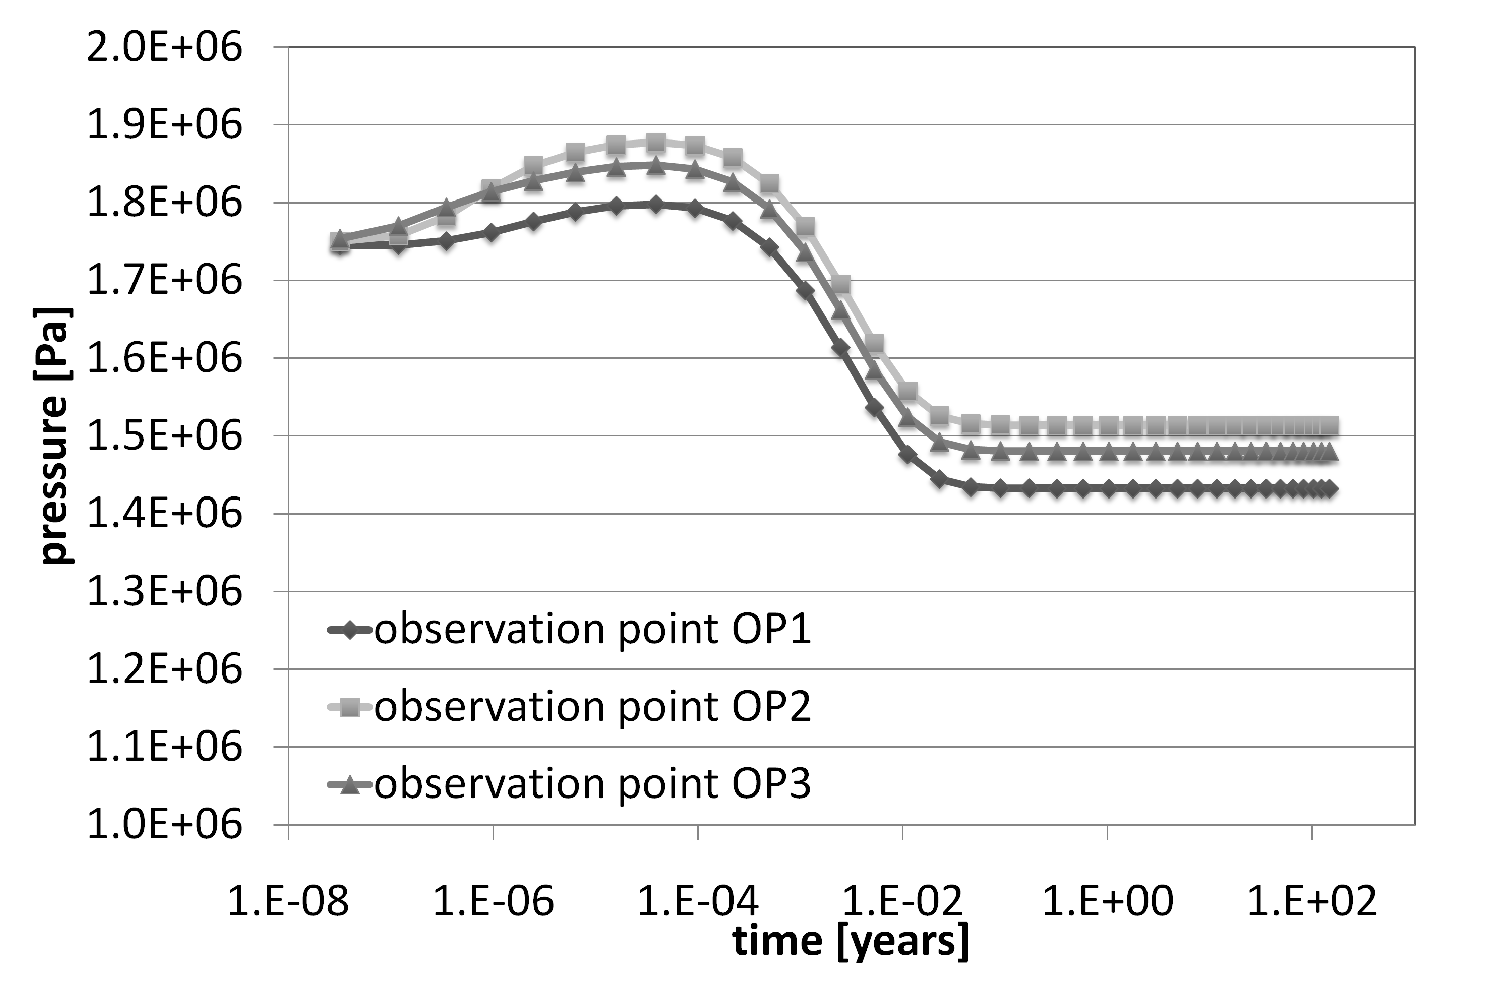
\includegraphics[width=1\textwidth]{T/figures/2u2f_fig6b.eps}
        \end{minipage}
        \begin{minipage}{0.40\textwidth}
            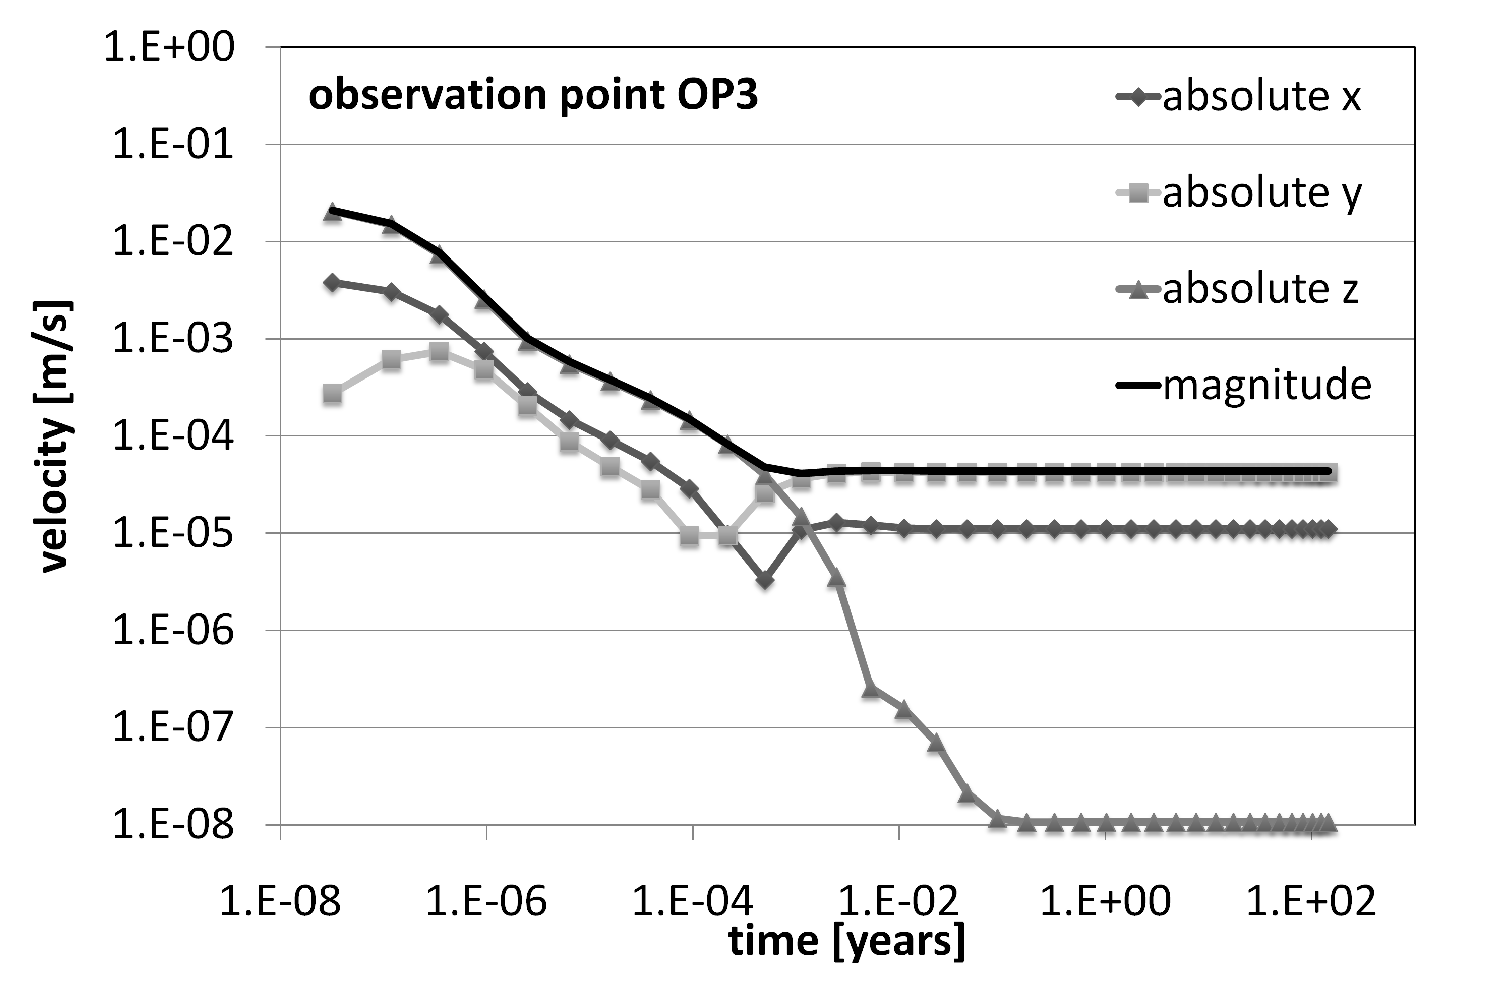
\includegraphics[width=1\textwidth]{T/figures/2u2f_fig6c.eps}
        \end{minipage}
        \begin{minipage}{0.40\textwidth}
            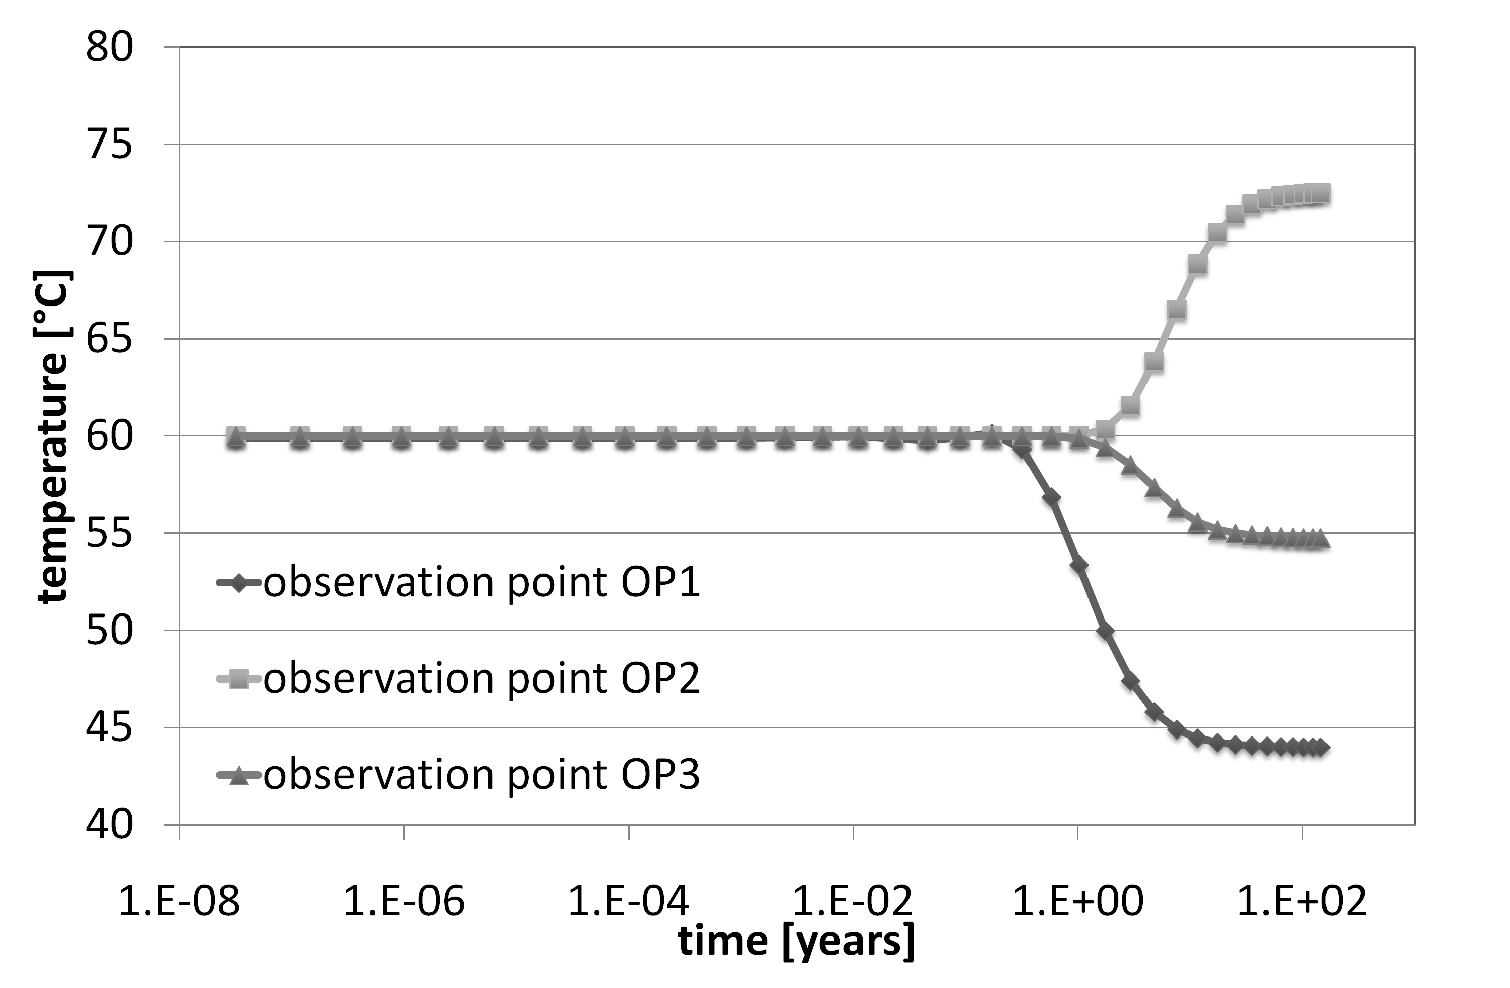
\includegraphics[width=1\textwidth]{T/figures/2u2f_fig6d.eps}
        \end{minipage}
        \caption{Location of three observation points within the fault faces (\ref{fig6}a); Simulated pressure (\ref{fig6}b) and temperature (\ref{fig6}d) values at these observation points and simulated velocity components (\ref{fig6}c) at observation point 3.}
        \label{fig6}
    \end{center}
\end{figure}

After starting the simulation the pressure increases at all observation points (Figure \ref{fig6}b). As shown for observation point 3 (Figure \ref{fig6}c), the initial magnitude of the velocity is due to vertical flow only. The observed downward flow is forced by the initial pressure conditions in combination with the chosen pressure boundary. Therefore, an initial increase of fluid pressure is observed. After 1 month, a stationary pressure and velocity field is reached, as indicated by the horizontal lines in Figure \ref{fig6}b-\ref{fig6}c.

The vertical component of velocity decreases over time from 3$\cdot10^{-2}$ m/s to $10^{-8}$ m/s, and the horizontal flow from the South to the North with velocities between $10^{-5}$ m/s and $10^{-4}$ m/s becomes dominant. The cold water reaches the fault system at the edge of fault 1 (Figure \ref{fig6}d) after approx. 4 month. After an additional 17 months, cooling at observation point 3 begins. At the same time, hot water reaches fault 2 first. Due to the lower transmissivity of fault 2, the hot water reaches the intersection point after 10 years, and cooling at observation point 3 stops. Higher amounts of cold water enter the fault intersection (observation point 3) from the more conductive fault 1, causing temperature to decrease to 55$^\circ{}$C. This corroborates the observation of the temperature field for the total domain.

In a second run, the same problem described above has been numerically solved using the Flux Corrected Transport (FCT) scheme as implemented in Norihiro's branch of OpenGeoSys version 5. Figure \ref{fig7} illustrates the differences regarding numerical oscillations in solving for the transport field with (dashed lines) and without (solid lines) FCT method. Figure \ref{fig7}a and Figure \ref{fig7}b show the calculated temperature profiles along the general flow field for two different stages in the simulation. As shown in Figure \ref{fig7}a, the FCT method seems to reduce the amplitudes of numerical oscillations by a maximum factor of three at the beginning of the simulation. The OGS benchmark files can be found in the subdirectory 2units2faults/FCT.
 
%figure7
\begin{figure}[htbp]
    \begin{center}
        \begin{minipage}{0.72\textwidth}
            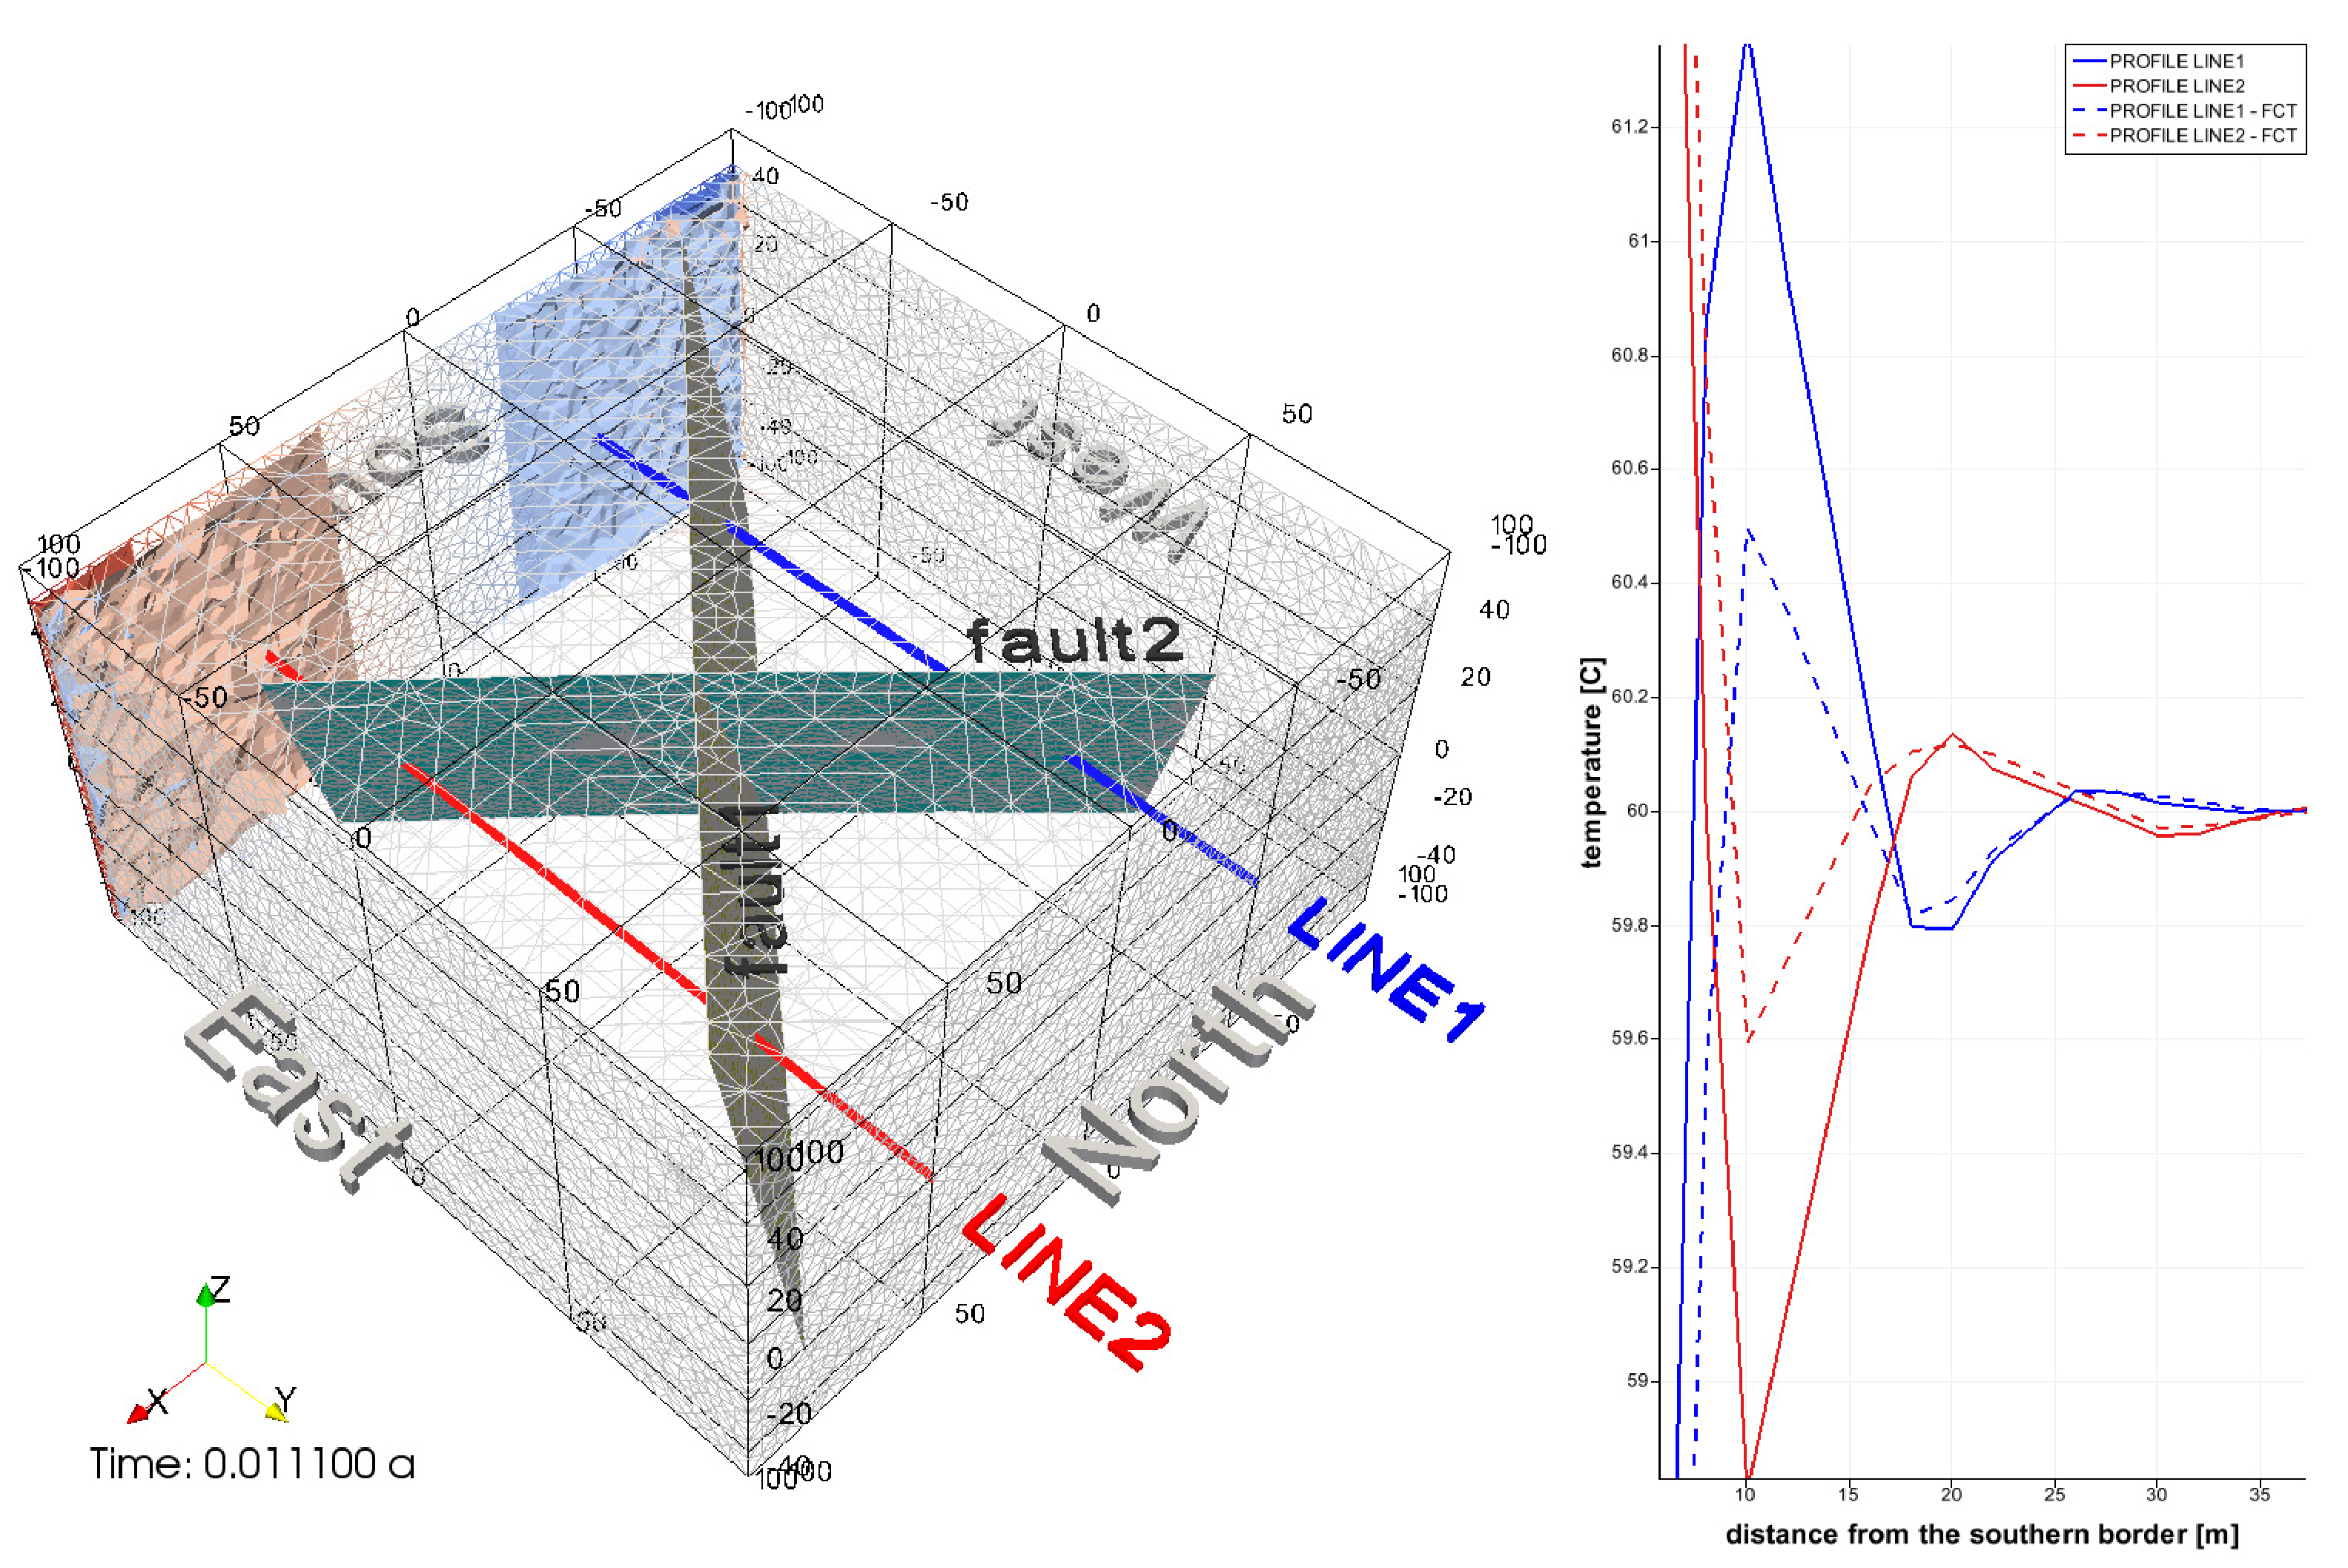
\includegraphics[width=1\textwidth]{T/figures/2u2f_fig7a.eps}
        \end{minipage}
        \begin{minipage}{0.72\textwidth}
            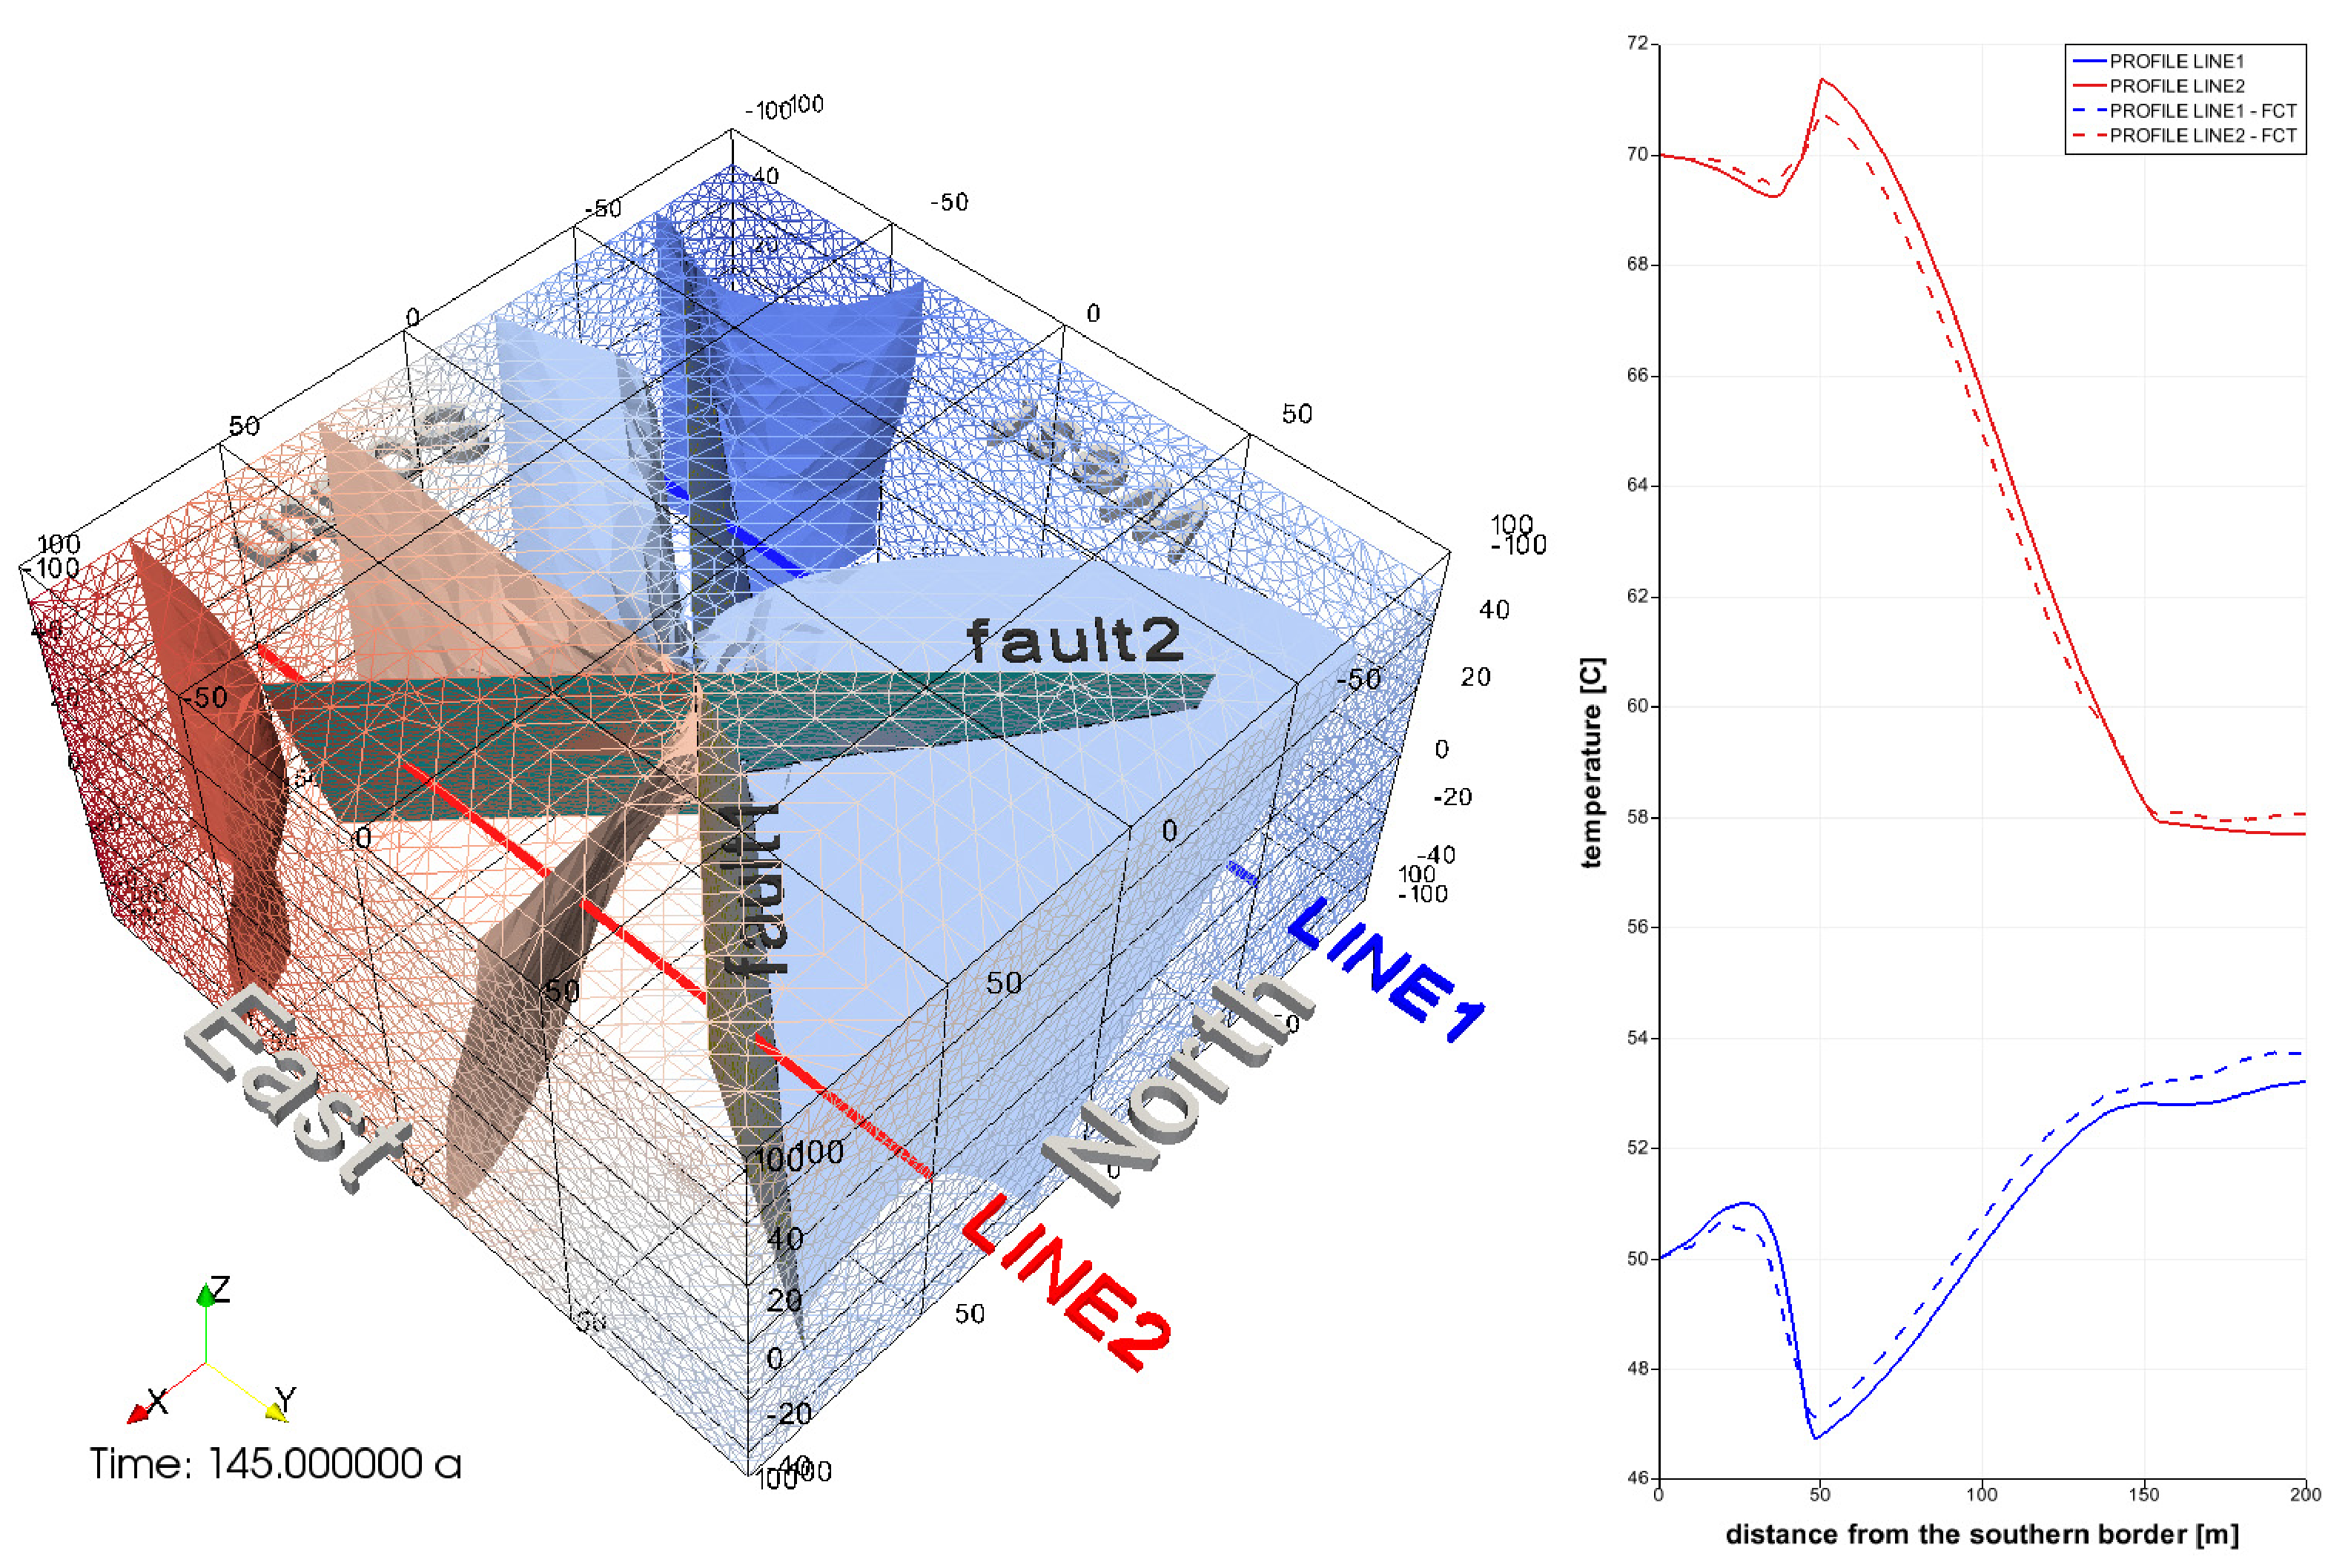
\includegraphics[width=1\textwidth]{T/figures/2u2f_fig7b.eps}
        \end{minipage}
        \caption{Simulated temperature along two lines at the beginning (\ref{fig7}a) and at the final simulation time (\ref{fig7}b) with and without flux corrected transport FCT.}
        \label{fig7}
    \end{center}
\end{figure}


